\section{三维坐标系与向量} \label{sec:3d-coord}

与二维平面类似, 在三维空间中我们通常使用直角坐标系来表示位置.
三维空间中还有两种比较常见的坐标系: 柱坐标系和球坐标系.

\subsection{空间直角坐标系}

空间直角坐标系是平面直角坐标系在三维空间中的扩展.
如图\ref{fig:xyz-coord},
它由三条两两垂直的坐标轴构成, 三条坐标轴有公共的原点$O$.
将三条坐标轴分别记作$x,y,z$轴, 任取两条坐标轴,
可以确定一个平面, 由此可以确定三个坐标平面,
分别记作$xOy,yOz,zOx$平面.
根据空间中一点$P$在$x,y,z$轴上的对应数值可以确定点$P$的位置,
这也就是点$P$的直角坐标.

\begin{figure}[htbp]
  \centering
  \begin{tikzpicture}[x=(-135:15mm),y=(-15:15mm),z=(90:15mm)]
    \draw[dashed] (0,0,0) -- (1,0,0);
    \draw[-latex] (1,0,0) -- (1.5,0,0) node[left] {$x$};
    \draw[dashed] (0,0,0) -- (0,2,0);
    \draw[-latex] (0,2,0) -- (0,2.5,0) node[right] {$y$};
    \draw[dashed] (0,0,0) -- (0,0,1.5);
    \draw[-latex] (0,0,1.5) -- (0,0,2) node[left] {$z$};
    \node[below] at (0,0,0) {$O$};

    \draw (1,2,0) -- (1,0,0) -- (1,0,1.5) -- (0,0,1.5)
    -- (0,2,1.5) -- (0,2,0) -- (1,2,0)
    -- (1,2,1.5) -- (0,2,1.5) (1,2,1.5) -- (1,0,1.5);

    \node[dot,label={below right,background:
          $P=(1,2,1.5)$}] at (1,2,1.5) {};
    \node[left] at (1,0,0) {1};
    \node[below] at (0,2,0) {2};
    \node[left] at (0,0,1.5) {1.5};
  \end{tikzpicture}
  \caption{空间直角坐标系}
  \label{fig:xyz-coord}
\end{figure}

根据$x,y,z$轴的相对位置,
三维坐标系分为\emph{左手坐标系}和\emph{右手坐标系}两种.
如图\ref{fig:xyz-hand}, 假设在屏幕中有一个空间坐标系,
我们旋转这个坐标系, 使得我们看向屏幕时,
$x$轴水平朝右, $y$轴竖直朝上, 这时$z$轴可能朝向屏幕里面或者外面.
如果$z$轴朝外, 则称之为右手坐标系;
如果$z$轴朝里, 则称之为左手坐标系.

\begin{figure}[htbp]
  \centering
  \begin{subfigure}{0.3\textwidth}
    \centering
    \begin{tikzpicture}[scale=2]
      \begin{scope}[-latex]
        \draw (0,0,0) -- (1,0,0) node[right] {$x$};
        \draw (0,0,0) -- (0,1,0) node[left] {$y$};
        \draw (0,0,0) -- (0,0,1) node[left] {$z$};
      \end{scope}
    \end{tikzpicture}
    \caption{右手坐标系}
  \end{subfigure}
  \begin{subfigure}{0.3\textwidth}
    \centering
    \begin{tikzpicture}[scale=2]
      \begin{scope}[-latex]
        \draw (0,0,0) -- (1,0,0) node[right] {$x$};
        \draw (0,0,0) -- (0,1,0) node[left] {$y$};
        \draw (0,0,0) -- (0,0,-1) node[right] {$z$};
      \end{scope}
    \end{tikzpicture}
    \caption{左手坐标系}
  \end{subfigure}
  \caption{}
  \label{fig:xyz-hand}
\end{figure}

左手坐标系和右手坐标系都有比较广泛的应用.
数学中通常使用右手坐标系,
常见的数学绘图工具比如Desmos, Geogebra都只有右手坐标系可用.
这大概是为了让$x,y$在水平面上, 然后用$z$表示垂直的高度.
而在游戏开发中左手坐标系很常见,
比如LuaSTG的道中背景制作, 使用的就是左手坐标系,
大概是为了让$x$轴向右, $y$轴向上时, 用$z$坐标表示垂直于屏幕向里的深度.

\begin{figure}[htbp]
  \centering
  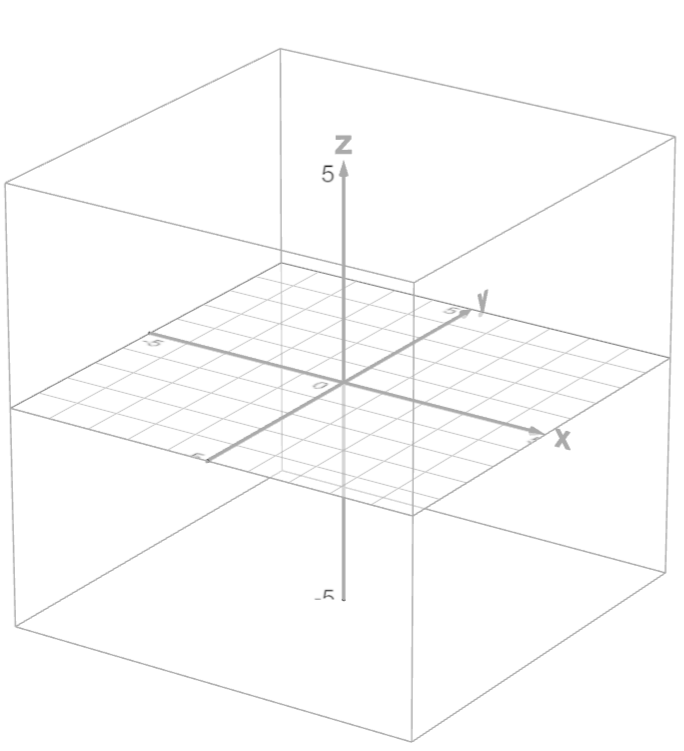
\includegraphics[width=0.3\textwidth]
  {assets/3d/desmos-3d.png}
  \caption{Desmos的3D绘图}
  \label{fig:desmos-3d}
\end{figure}

\subsection{柱坐标系和球坐标系}

如下图所示, 柱坐标系用$xOy$平面上的极坐标$r,\theta$,
以及$z$轴上的坐标$z$确定点的位置.
柱坐标与直角坐标的转换就是$xOy$上的极坐标与直角坐标的转换,
没什么好说的.
\[
  \begin{cases}
    x = r\cos\theta \\
    y = r\sin\theta \\
    z = z
  \end{cases}\quad\quad\quad
  \begin{cases}
    r = \Dist(0,0,x,y)       \\
    \theta = \Angle(0,0,x,y) \\
    z = z
  \end{cases}
\]

\begin{center}
  \begin{tikzpicture}[x=(-135:15mm),y=(-15:15mm),z=(90:15mm)]
    \draw[-latex] (0,0,0) -- (1.5,0,0) node[left] {$x$};
    \draw[-latex] (0,0,0) -- (0,1.5,0) node[right] {$y$};
    \draw[-latex] (0,0,0) -- (0,0,1.5) node[left] {$z$};

    \path (1,0,0) -- (0,0,0) node[above,sloped,midway] {$r$};
    \begin{scope}[canvas is xy plane at z=0]
      \draw (1,0) arc (0:60:1) -- (0,0);
      \draw[->] (2mm,0) arc (0:60:2mm)
      node[midway,below] {$\theta$};
    \end{scope}
    \draw (60:1) -- +(0,0,1.5)
    node[dot,label={right:$(r,\theta,z)$}] {}
    node[midway,right] {$z$};
  \end{tikzpicture}
\end{center}

球坐标系通过球面半径和点在球面上的角来确定点在空间中的位置.
不同资料对球坐标的具体定义有所不同,
本教程采用地理中经纬度的概念来进行定义.
对于空间中的一点$P$, 作一个以原点为球心, 经过点$P$的球面.
设球面的半径为$\rho$, 点$P$在球面上的经度为$\theta$,
纬度为$\phi$ ($-90\degree \le \phi \le 90\degree$).
由$\rho,\theta,\phi$可以确定点$P$的位置.

\begin{center}
  \begin{tikzpicture}[x=(-135:15mm),y=(-15:15mm),z=(90:15mm)]
    \draw[-latex] (0,0,0) -- (1.5,0,0) node[left] {$x$};
    \draw[-latex] (0,0,0) -- (0,1.5,0) node[right] {$y$};
    \draw[-latex] (0,0,0) -- (0,0,1.5) node[left] {$z$};

    \begin{scope}[canvas is xy plane at z=0]
      \draw (1,0) arc (0:75:1) -- (0,0);
      \draw (2mm,0) arc (0:75:2mm)
      node[midway,below] {$\theta$};
    \end{scope}

    \begin{scope}[
        plane x={(75:1)},
        plane y={(0,0,1)},
        canvas is plane,
      ]
      \draw (1,0) arc (0:80:1) coordinate (P);
      \draw (2mm,0) arc (0:80:2mm)
      node[midway,right,background] {$\phi$};
    \end{scope}

    \draw (0,0,0) -- (P) node[dot,label={
          right:$(\rho,\theta,\phi)$}] {};
  \end{tikzpicture}
\end{center}

球坐标$(\rho,\theta,\phi)$与直角坐标$(x,y,z)$有如下转换关系:
\[
  \begin{cases}
    x = \rho\cos\phi \cdot \cos\theta \\
    y = \rho\cos\phi \cdot \sin\theta \\
    z = \rho\sin\phi
  \end{cases}\quad\quad\quad
  \begin{cases}
    \rho = \sqrt{x^2+y^2+z^2} \\
    \theta = \Angle(0,0,x,y)  \\
    \phi = \arcsin\dfrac{z}{\rho}
  \end{cases}
\]

\section{三维向量}

我们在第二章所讲的关于向量的大部分内容可以直接用到三维向量上,
比如向量的几何意义, 线性运算, 线性变换等.
这里我们补充一下三维向量的内积和外积.

三维向量的内积与二维差不多, 向量
$\vec r_1=(x_1,y_1,z_1),\ \vec r_2=(x_2,y_2,z_2)$
的内积为
\[
  \vec r_1 \cdot \vec r_2 = x_1x_2 + y_1y_2 + z_1z_2.
\]

内积的几何意义也差不多, 设$\vec r_1,\vec r_2$的夹角为
$\theta$ ($0\degree \le \theta \le 180\degree$), 则有
\[
  \vec r_1 \cdot \vec r_2 = |\vec r_1|\cdot|\vec r_2| \cos\theta.
\]

两个三维向量的外积是一个新的三维向量.
设三维向量$\vec r_1,\vec r_2$的外积为
$\vec r_3 = \vec r_1\times\vec r_2$,
则有以下性质:

\begin{enumerate}
  \item $\vec r_3$的长度是确定的:
        设$\vec r_1,\vec r_2$的夹角为$\theta$
        ($0\degree \le \theta \le 180\degree$), 则有
        \[
          |\vec r_3| = |\vec r_1|\cdot|\vec r_2|\cdot|\sin\theta|.
        \]
  \item $\vec r_3$的方向是确定的.
        $\vec r_3$垂直于$\vec r_1$和$\vec r_2$ (构成的平面)
        \footnote{
          如果$\vec r_1,\vec r_2$共线,
          那么$\vec r_1\times\vec r_2$的长度为0,
          不用考虑其方向.
        }.
        如下图, 如果使用右手坐标系,
        那么$\vec r_1,\vec r_2,\vec r_3$也构成右手系.
        左手坐标系同理.

        \begin{center}
          \begin{tikzpicture}[
              x=(-135:7mm),y=(0:10mm),z=(90:10mm)
            ]
            \begin{scope}[
                plane x={(1,0,0)},
                plane y={(0,1,0)},
                canvas is plane,
              ]
              \fill[blue!10] (-2.5,-2.5) rectangle (2.5,2.5);
            \end{scope}

            \begin{scope}[-latex]
              \draw (0,0,0) -- (2.5,0,0) node[left] {$x$};
              \draw (0,0,0) -- (0,2.5,0) node[right] {$y$};
              \draw (0,0,0) -- (0,0,2.5) node[left] {$z$};
            \end{scope}

            \coordinate (a) at (1.5,1,0);
            \coordinate (b) at (1,2,0);
            \coordinate (c) at (0,0,1.5);

            \begin{scope}[->]
              \draw (0,0,0) -- (a) node[below] {$\vec r_1$};
              \draw (0,0,0) -- (b) node[below] {$\vec r_2$};
              \draw (0,0,0) -- (c) node[left] {$\vec r_3$};
            \end{scope}
          \end{tikzpicture}
        \end{center}

        特别地, 设$x,y,z$轴的单位向量为$\vec i,\vec j,\vec k$, 则有
        \[
          \vec i\times\vec j = \vec k,\quad
          \vec j\times\vec k = \vec i,\quad
          \vec k\times\vec i = \vec j.
        \]
  \item 反交换律和线性性, 与二维向量的外积相同.
\end{enumerate}

设$\vec r_1=(x_1,y_1,z_1),\vec r_2=(x_2,y_2,z_2)$,
则外积$\vec r_1\times\vec r_2$的计算结果为
\[
  \vec r_1\times\vec r_2 =
  (y_1z_2 - y_2z_1, z_1x_2 - z_2x_1, x_1y_2 - x_2y_1).
\]
三个分量对应三组二维向量的外积, 比如$x$坐标,
是$\vec r_1,\vec r_2$在$yOz$平面上的投影
$(y_1,z_1),(y_2,z_2)$的外积, $y,z$坐标同理.
